\section{Software}

\subsection{Umfang}

Im Rahmen des Projektes wurde eine Android-Applikation entwickelt. Diese läuft ab der Androidversion 4.3 (API Level 18). Mit der Applikation können Servicetechniker Küchenaufbauten protokollieren und die Parametrisierung der Geräte auslesen und bearbeiten.

Die App wurde von der Firma Fluxron AG übernommen und wird dort weiterentwickelt und in den App Store publiziert.

\subsection{Package-Struktur}

Die Software basiert auf einem Schichtenmodell, bei welchem die Schichten mittels einem Event Bus verbunden werden. Zudem gibt es einen Applikationskontext, Pakete mit Meldungstypen und ein Paket mit den Datenobjekten. 

\begin{figure}[H]
    \begin{center}
    		% GFX Trim left bottom right top
        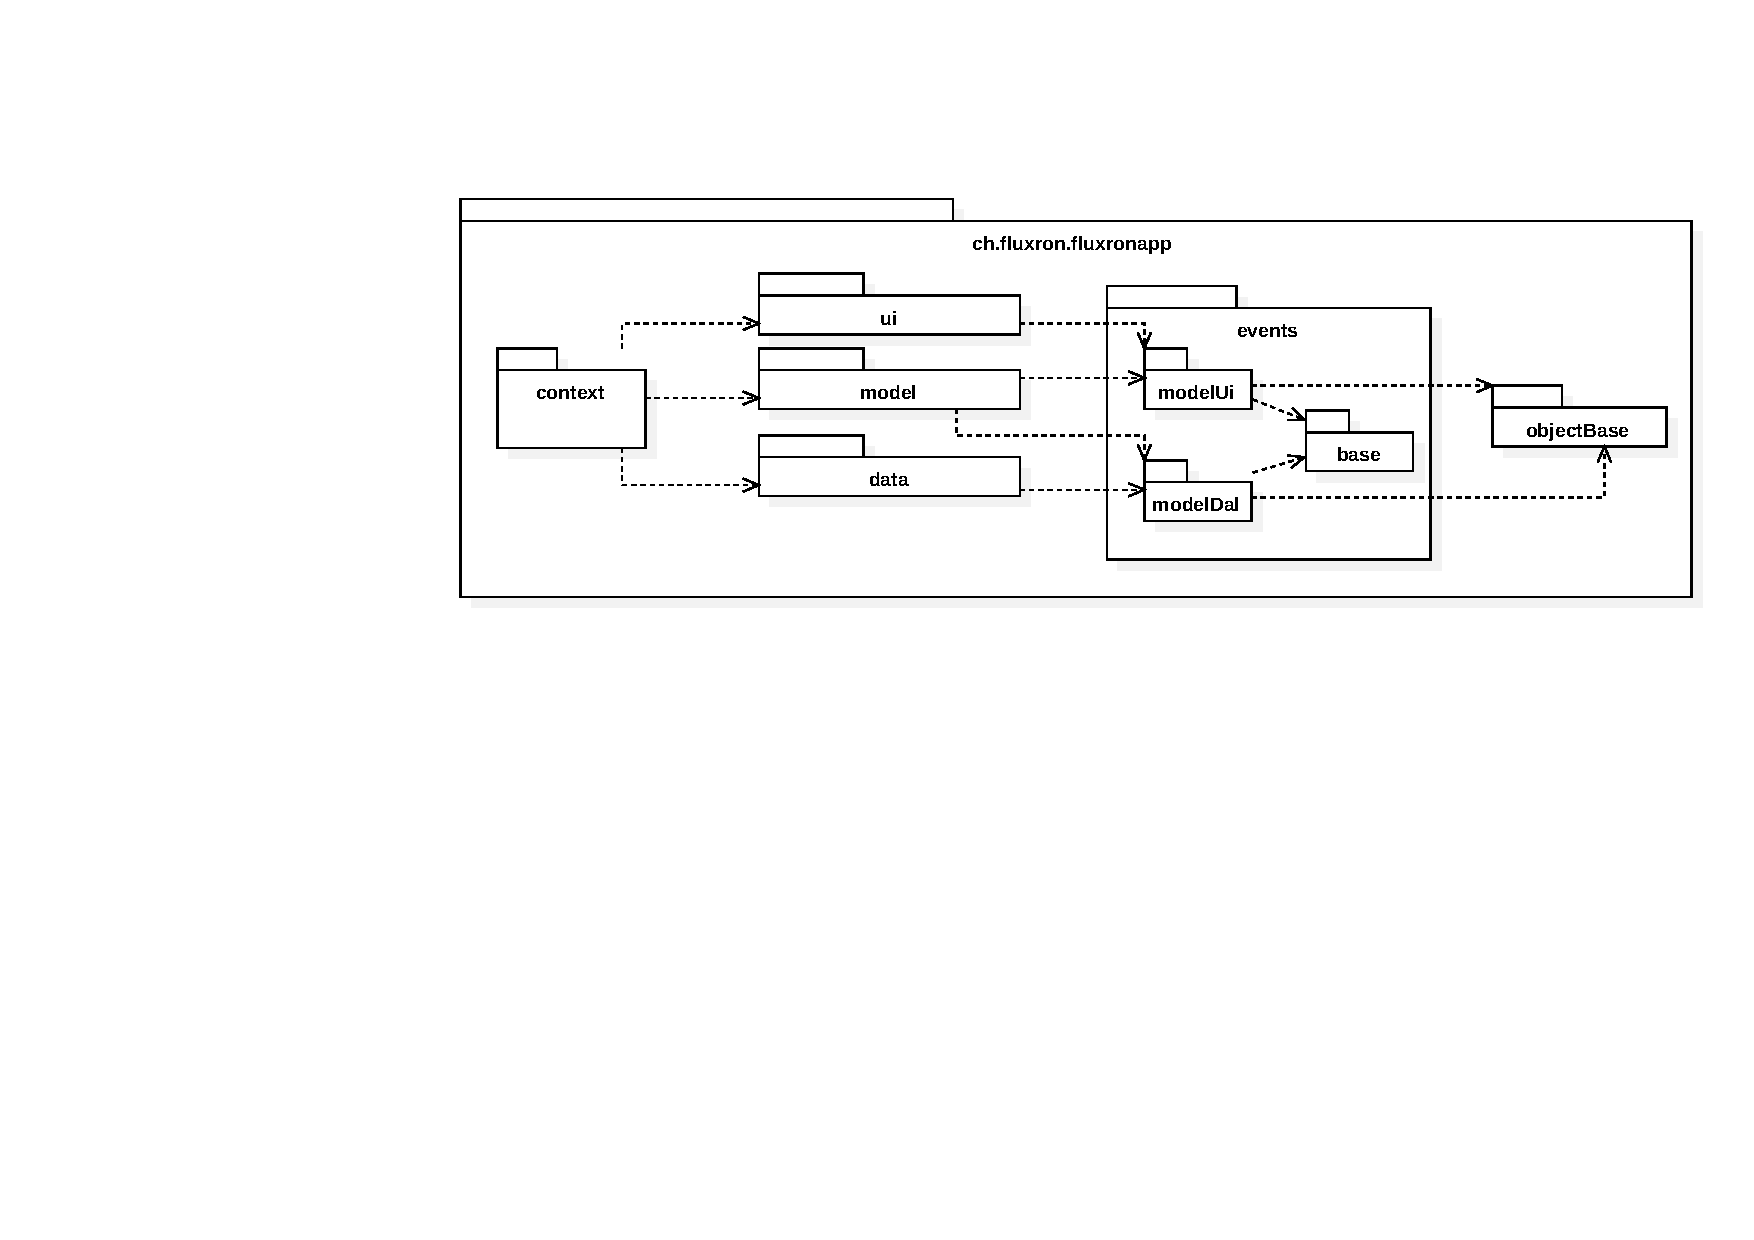
\includegraphics[trim=220 300 0 90,clip,scale=0.7]{results/res/package_diagram}
    \end{center}
    \caption{Packagediagramm der App}
    \label{abb:packages}
\end{figure}

\subsubsection{ch.fluxron.fluxronapp.context}
Dieses Paket enthält den Applikationskontext. Dieser wird beim Starten der Applikation initialisiert und beinhaltet sowohle den Event Bus für die Kommunikation zwischen Model und User Interface, als auch den Bus zwischen Data und Model. Die Referenzen auf den jeweiligen Event Bus werden über Dependency Injection an die, ebenfalls im Kontext initialisierten, Listenerklassen aus Model und Data weitergegeben.

\subsubsection{ch.fluxron.fluxronapp.ui}
Beinhaltet alle UI-Klassen. Dies sind Activities, Fragments, Custom Views, Animationen und Listenadapter. Diese Klassen haben alle direkt mit dem User Interface und der Anzeigelogik zu tun.

\subsubsection{ch.fluxron.fluxronapp.model}
In diesem Paket sind die Logikklasen des Businessmodells gebündelt. Sie alle haben gemeinsam, dass sie Meldungen von der Benutzeroberfläche verarbeiten und an die Datenschicht weiterleiten, oder umgekehrt.

\subsubsection{ch.fluxron.fluxronapp.data}
Dieses Paket besteht aus zwei Hauptbereichen: Die lokale Datenbankanbindung mittels Couchbase Lite und die Bluetooth-Schnittstelle. Beide Bereiche erhalten Meldungen von der Logikschicht und lösen selbst Meldungen aus (z.B. ein Gerät wurde gefunden).

\subsubsection{ch.fluxron.fluxronapp.events}
Die gesamte Kommunikation zwischen den Layern basiert auf Event- und Meldungsklassen. Diese sind in diesem Paket in drei Unterpakete gegliedert.

Das Paket \textbf{modelUi} enthält Nachrichten, welche zwischen Benutzeroberfläche und Logik ausgetauscht werden.

Im Package \textbf{modelDal} befinden sich Meldungstypen, die für die Kommunikation zwischen Logik, Datenbank und Bluetooth-Schnittstelle versendet werden.

Beide Meldungsgruppen basieren auf den Klassen aus \textbf{base}. Diese implementieren grundlegende Mechanismen wie z.B. Request-Reply Pattern oder das synchrone warten auf Antworten auf eine Meldung.

\subsubsection{ch.fluxron.fluxronapp.objectBase}
Für den Nachrichtenaustausch und die Speicherung der Daten werden noch Datenobjekte benötigt. Diese sind häufig Bestandteil einer Meldung und werden somit von vielen Meldungsklassen referenziert.

\subsubsection{Laufzeitstruktur}
\begin{figure}[H]
    \begin{center}
    		% GFX Trim left bottom right top
        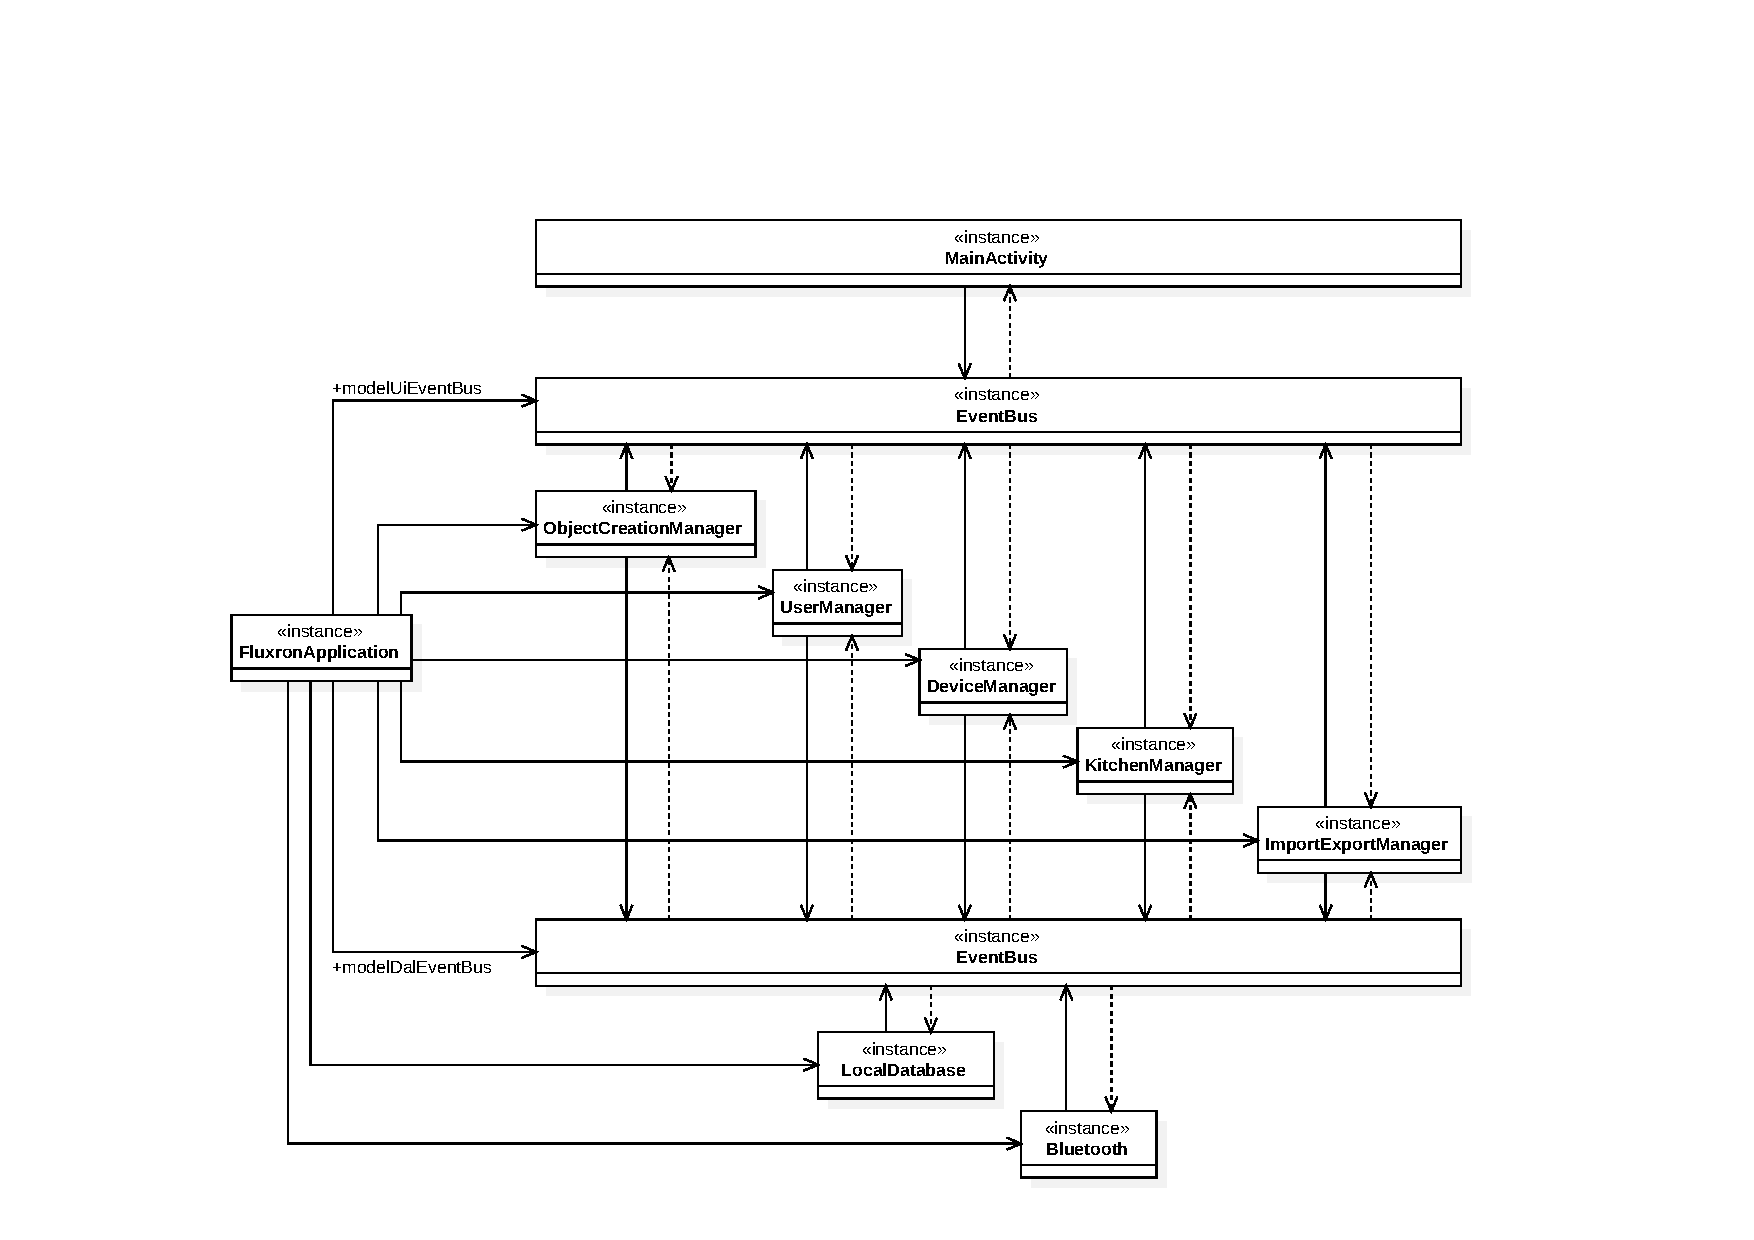
\includegraphics[trim=100 30 0 90,clip,scale=0.7]{results/res/instances}
    \end{center}
    \caption{Laufzeitstruktur der App}
    \label{abb:instances}
\end{figure}

Beim Start der Applikation wird der Kontext (FluxronApplication) durch das Betriebssystem  erzeugt. Dieser erstellt dann die beiden Event Bus Objekte und erzeugt auch die Instanzen der Manager- und Datenklassen. Dies ist notwendig, da sich die Layer gegenseitig nicht kennen und nur über einen Event Bus miteinander kommunizieren können. Die Instanzierung aller Manager muss direkt zu Beginn der Applikation gemacht werden, damit sich die Instanzen beim Event Bus registrieren können.

Jede Managerklasse hat eine Assoziation mit dem Event Bus (Aufruf des Meldungsversandes) und wird durch diesen aufgrund der Subscription referenziert.

\subsubsection{Nachrichtenfluss}
Nachrichten werden auf mehrere Arten genutzt, um die Verbindung zwischen den Layern herzustellen:

\begin{itemize}
\item{Versenden von Befehlen z.B. SaveKitchenCommand}
\item{Kontextlose Ereignismeldungen z.B. DeviceFound}
\item{Antworten auf Befehle z.B. ResponseOK}
\end{itemize}

Nachfolgend ist der Nachrichtenverlauf am Beispiel \enquote{Ändern im Fehlerfall} abgebildet.

\begin{figure}[H]
    \begin{center}
    		% GFX Trim left bottom right top
        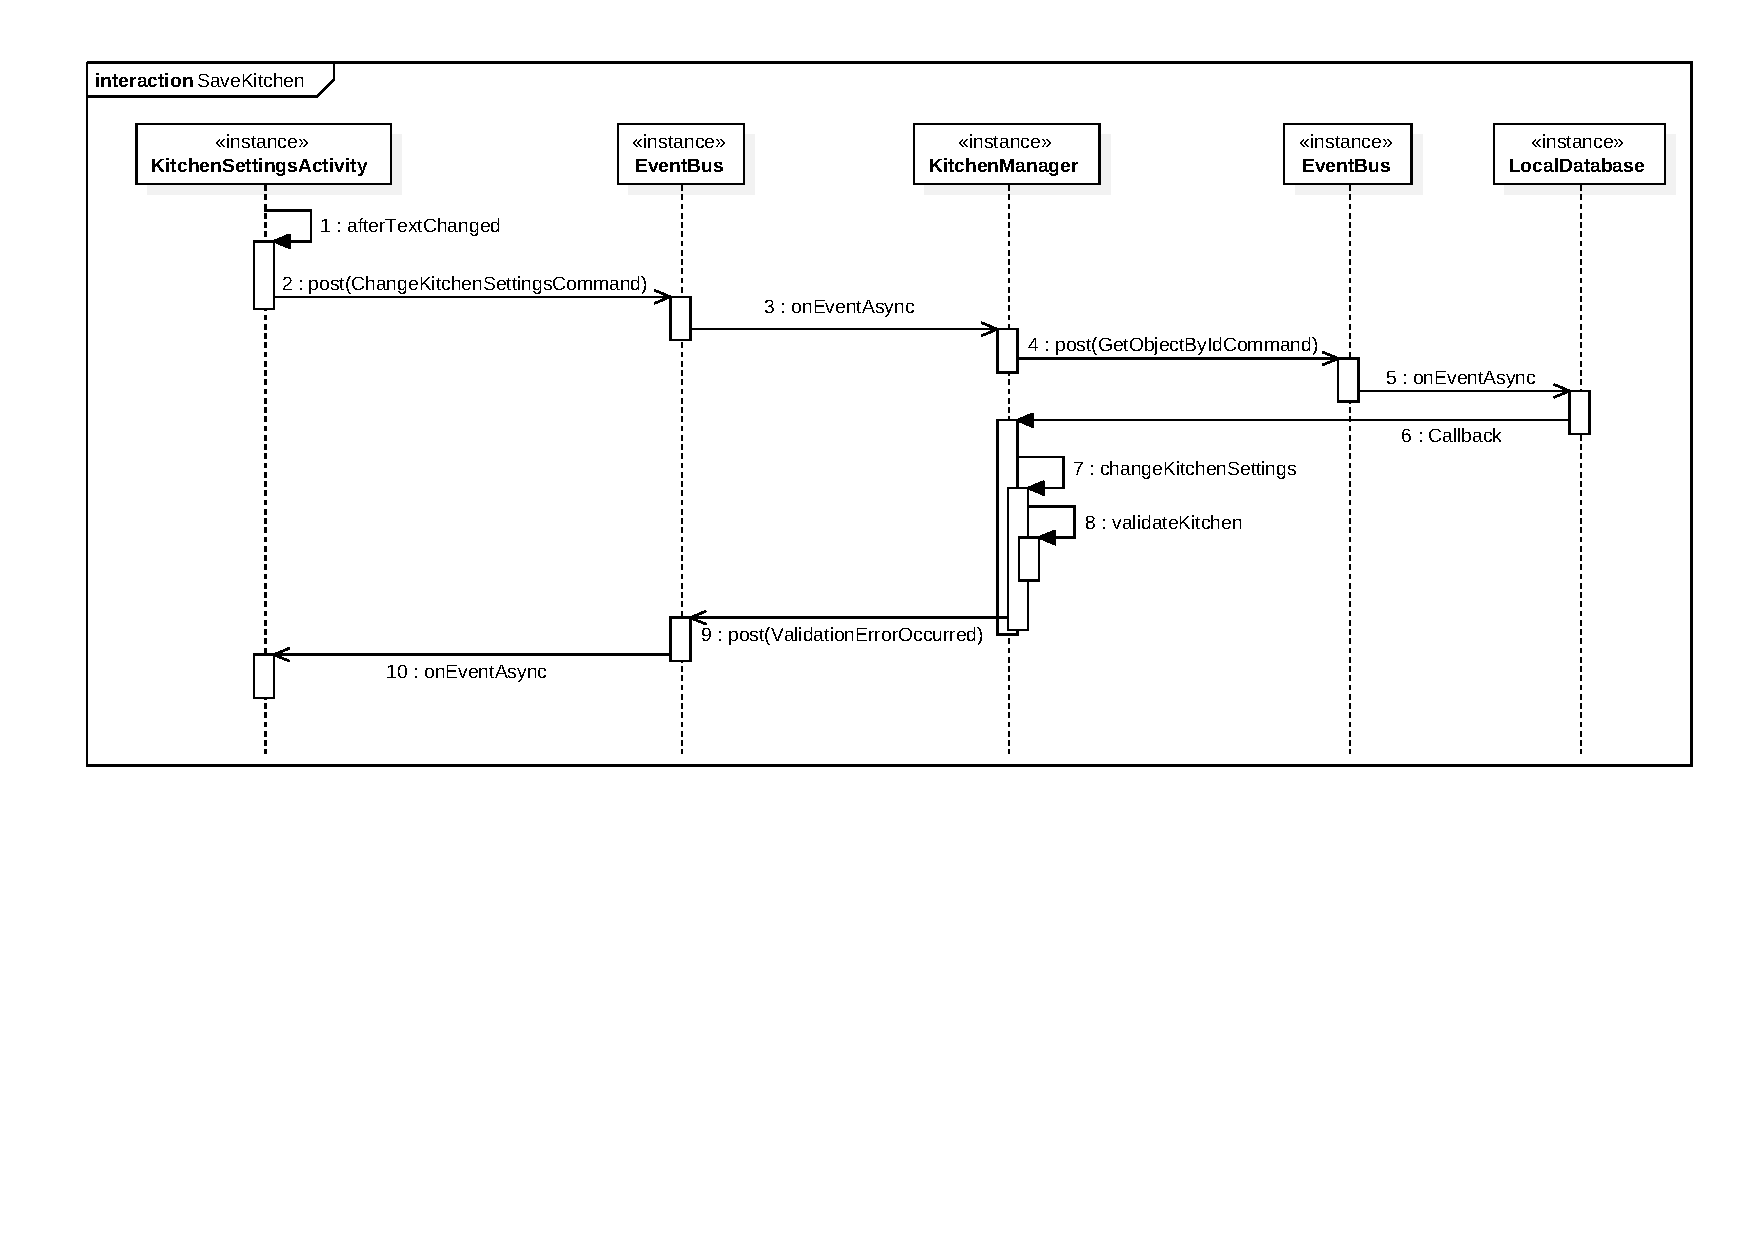
\includegraphics[trim=40 225 30 30,clip,scale=0.55]{results/res/messages}
    \end{center}
    \caption{Meldungsverlauf beim Ändern von Kücheneinstellungen mit Validierungsfehlern}
    \label{abb:messages}
\end{figure}

\begin{enumerate}
\item{Benutzeroberfläche registriert eine Textänderung}
\item{Wertänderung Name wird als Befehl über den Event Bus versendet}
\item{Bus verteilt die Meldung an alle Listener}
\item{Ladebefehl für die Küche anhand Id}
\item{LocalDatabase empfängt Ladebefehl}
\item{Callback, wird aufgerufen, sobald das Objekt geladen ist}
\item{Einstellungen des geladenen Objekts werden angepasst}
\item{Validierung der Werte}
\item{Aufgetretene Fehlermeldungen werden als Event über den Bus versendet}
\item{Meldung trifft bei Benutzeroberfläche ein, Fehler wird dargestellt}
\end{enumerate}

\subsection{Codestatistik}

Zur Überprüfung der Codestatistik wurde neben Codereviews auch Codestatistiken ausgewertet. Nachfolgend ist die Statistik für das Projektende aufgeführt. Alle gemessenen Werte befinden sich im erwarteten und grünen Bereich. Im Schnitt zeigen diese Werte eine gute Wartbarkeit und Qualität des entwickelten Programms.

Bei einzelnen Klassen sind Abweichungen vom Durchschnitt festzustellen. Diese lassen sich aber alle begründen. So sind zum Beispiel die Werte für die \enquote{Lack of Cohesion of Methods} der Plain Old Java Objects sehr hoch, denn diese bestehen nur aus Gettern und Settern.

\subsubsection{Class Metrics}

\begin{table}[H]
	\begin{center}
	  \begin{tabular}{ | l | r | }
	    \hline
	    \textbf{Metrik} & \textbf{Wert} \\ \hline
	    (Avg) Coupling Between Objects & 7.30\\ \hline
   	    (Avg) Depth of Inheritance & 2.35 \\ \hline
   	    (Avg) Lack of Cohesion of Methods & 2.04 \\ \hline
  	    (Avg) Weighted Method Complexity & 9.34 \\ \hline
  	    Number of Product Plasses & 217.00 \\ \hline
	  \end{tabular}
	  \caption{Class Metrics für ch.fluxron.fluxronapp}
  \end{center}
\end{table}

\subsubsection{Complexity Metrics}

\begin{table}[H]
	\begin{center}
	  \begin{tabular}{ | l | r | }
	    \hline
	    \textbf{Metrik} & \textbf{Wert} \\ \hline
	    (Avg) Method Cyclomatic Complexity & 1.56 \\ \hline
  	    (Avg) Method Lines Of Code & 11.69 \\ \hline
  	    (Avg) Comment to Code Ratio & 38.56 \\ \hline
  	    (Avg) Javadoc Lines per Method & 4.23 \\ \hline
	  \end{tabular}
	  \caption{Complexity Metrics für ch.fluxron.fluxronapp}
  \end{center}
\end{table}

\subsubsection{Dependency Metrics}

\begin{table}[H]
	\begin{center}
	  \begin{tabular}{ | l | r | }
	    \hline
	    \textbf{Metrik} & \textbf{Wert} \\ \hline
	    (Avg) Number of Cyclic Dependencies & 0.00 \\ \hline
  	    (Avg) Number of Class Dependencies & 4.33 \\ \hline
  	    (Avg) Number of Package Dependencies & 0.96 \\ \hline
	  \end{tabular}
	  \caption{Complexity Metrics für ch.fluxron.fluxronapp}
  \end{center}
\end{table}